
\documentclass{article} % Don't change this

\usepackage[english]{babel}
\usepackage[utf8]{inputenc}
\usepackage[margin=1.2in]{geometry}
\usepackage{amsmath}
\usepackage{amsthm}
\usepackage{amsfonts}
\usepackage{multirow}
\usepackage{amssymb}
\usepackage{multicol}
\usepackage{booktabs}
\usepackage[usenames,dvipsnames]{xcolor}
\usepackage{graphicx}
\usepackage[siunitx]{circuitikz}
\usepackage{tikz}
\usepackage{lscape}
\usepackage[colorinlistoftodos, color=orange!50]{todonotes}
\usepackage{hyperref}
\usepackage[authoryear]{natbib}
\setcitestyle{authoryear,open={(},close={)}}
\usepackage{fancybox}
\usepackage{epsfig}
\usepackage{soul}
\usepackage{listings}
\usepackage{subcaption}
\lstset{language=[90]Fortran,
  basicstyle=\ttfamily,
  keywordstyle=\color{red},
  commentstyle=\color{green},
  morecomment=[l]{!\ }% Comment only with space after !
}

\usepackage{booktabs}
\setlength{\marginparwidth}{3.4cm}

%#########################################################

%To use symbols for footnotes
\renewcommand*{\thefootnote}{\fnsymbol{footnote}}
\newcommand{\tp}{\texttt}
%To change footnotes back to numbers uncomment the following line
%\renewcommand*{\thefootnote}{\arabic{footnote}}

% Enable this command to adjust line spacing for inline math equations.
% \everymath{\displaystyle}

\title{\raggedright
\normalfont \normalsize 
\huge Multi-threaded Programming: Scheduling and Affinity Coursework \\[1em]
\normalsize \normalfont Jack Tyler: 27513556 \\
\rule{\linewidth}{.5pt}  \\[6pt]
}

\begin{document}

\maketitle

In the early days of computing, computational power progressed at an alarming rate; constant field scaling meant that transistors could be fabricated smaller and smaller, allowing them to use less power, and for the clock speed of a processor to be increased.
However, transistor manufacture has hit a physical limit for scaling \citep{Mcfarland1995}, and as such, increasing the clock speed any further would require highly capable cooling solutions impractical for use.
As a result, processor companies have had to find other methods to speed up computer processors, to keep computational power, and Moore's Law, advancing.
Perhaps most prominent is the introduction of parallelism, where multiple processor units may exist on a processor `chip' and execute asynchronously and independently.

This type of parallelism is one of the most common implementations currently used in high-performance computing, to decrease program execution time.
However, care must be taken as to how each processor unit -- each thread -- is synchronised to complete a computational task in unison, and in particular,
some methods of synchronisation, or scheduling, may provide better performance for a particular application.

This report investigates the most effective scheduling algorithm for a particular computational problem on the ARCHER supercomputing cluster.
In particular, it studies the effectiveness of scheduling algorithms provided by the OpenMP standard, compared to a static partitioned affinity schedule work-stealing algorithm, specifically designed for the computation problem at hand, and identifies many of the limitations and shortcomings in both the paralellisation of the algorithm, and in the analysis method. Knowledge of the OpenMP standard and parallel computing nomenclature is assumed in this report.

\section*{Introduction to the Problem}

The problem statement for this work is, at first glance, straightforward: to parallelise two examplar computation loops, and investigate the effect of OpenMP-standard scheduling algorithms, or indeed a third-party algorithm, on program runtime.
However, it's worthwhile to first understand and consider potential approaches and pitfalls that may be experienced from an examination of the loop structures.

\begin{figure}
    \begin{lstlisting}
        do i = 1,N

            do j = N,i,-1
        
                a(j,i) = a(j,i) + cos(b(j,i))
        
            end do
      
        end do
    \end{lstlisting}
    \caption{Loop 1; note that this loop is well-balanced, and we should expect each thread to perform approximately the same amount of work for this loop.}
    \label{listing:loop1}
\end{figure}

Loop 1 (Figure \ref{listing:loop1}) is a simple, yet relatively imbalanced nested do-loop; each repetition of the inner do-loop is variable based on the value of \texttt{i}.
As a result, threads that are assigned a different value of \tp{i} will perform a different amount of work (Figure \ref{fig:loop1work}).
We might therefore expect scheduling algorithms that work well with a slight work imbalance to perform well on this problem, such as \tp{STATIC, \textit{n}}, \tp{GUIDED,\textit{n}}, or \tp{DYNAMIC,\textit{n}}. However, since the distribution of work is readily predictable, we may see good performance from the \tp{AUTO} option, which gives the compiler the authority to change the scheduling algorithm as it sees fit (including during runtime).

\begin{figure}
    \centering
    \begin{subfigure}{0.45\textwidth}
        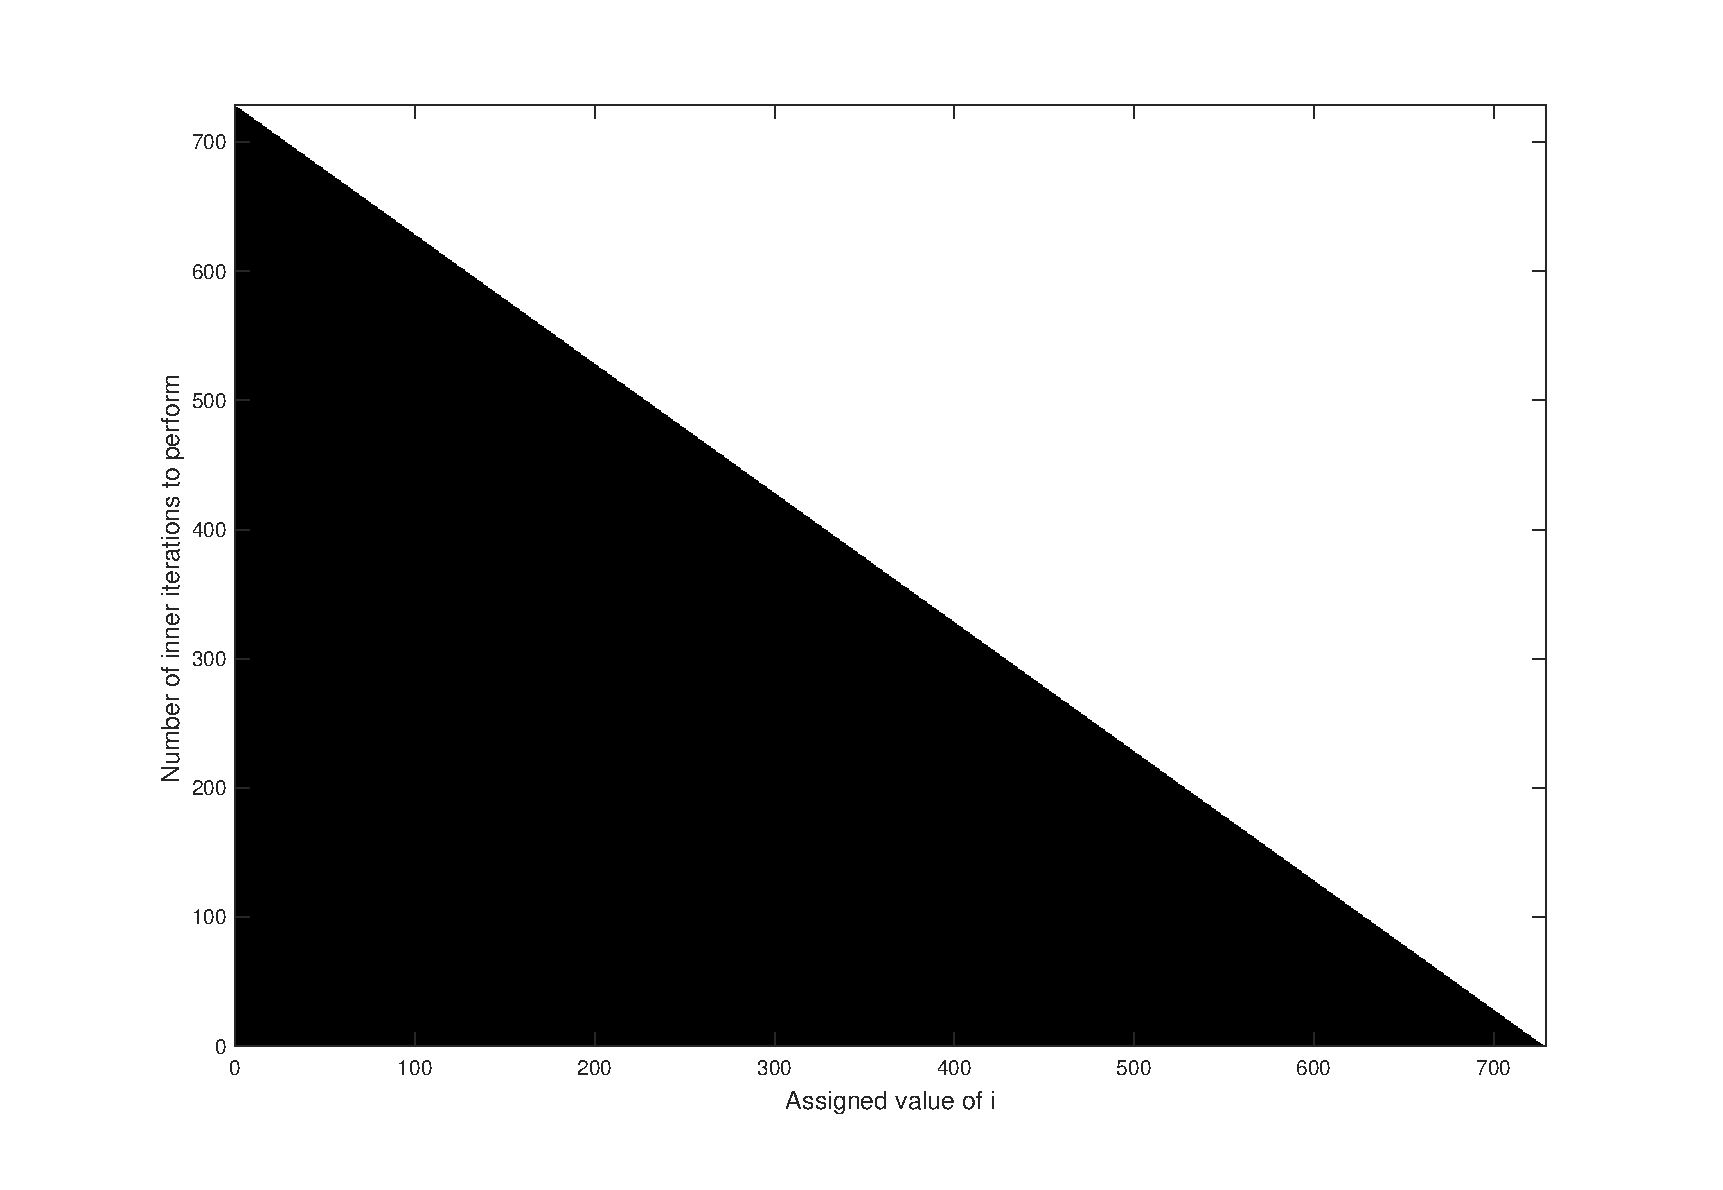
\includegraphics[width=\linewidth]{part1_plots/loop1_balancing.eps}
        \caption{The number of inner-loop iterations in Loop 1 a thread must perform based on the value of \tp{i} it is assigned; while this is a slight work imbalance, the number of iterations to perform is readily predictable.}
        \label{fig:loop1work}
    \end{subfigure}
    \begin{subfigure}{0.45\textwidth}
        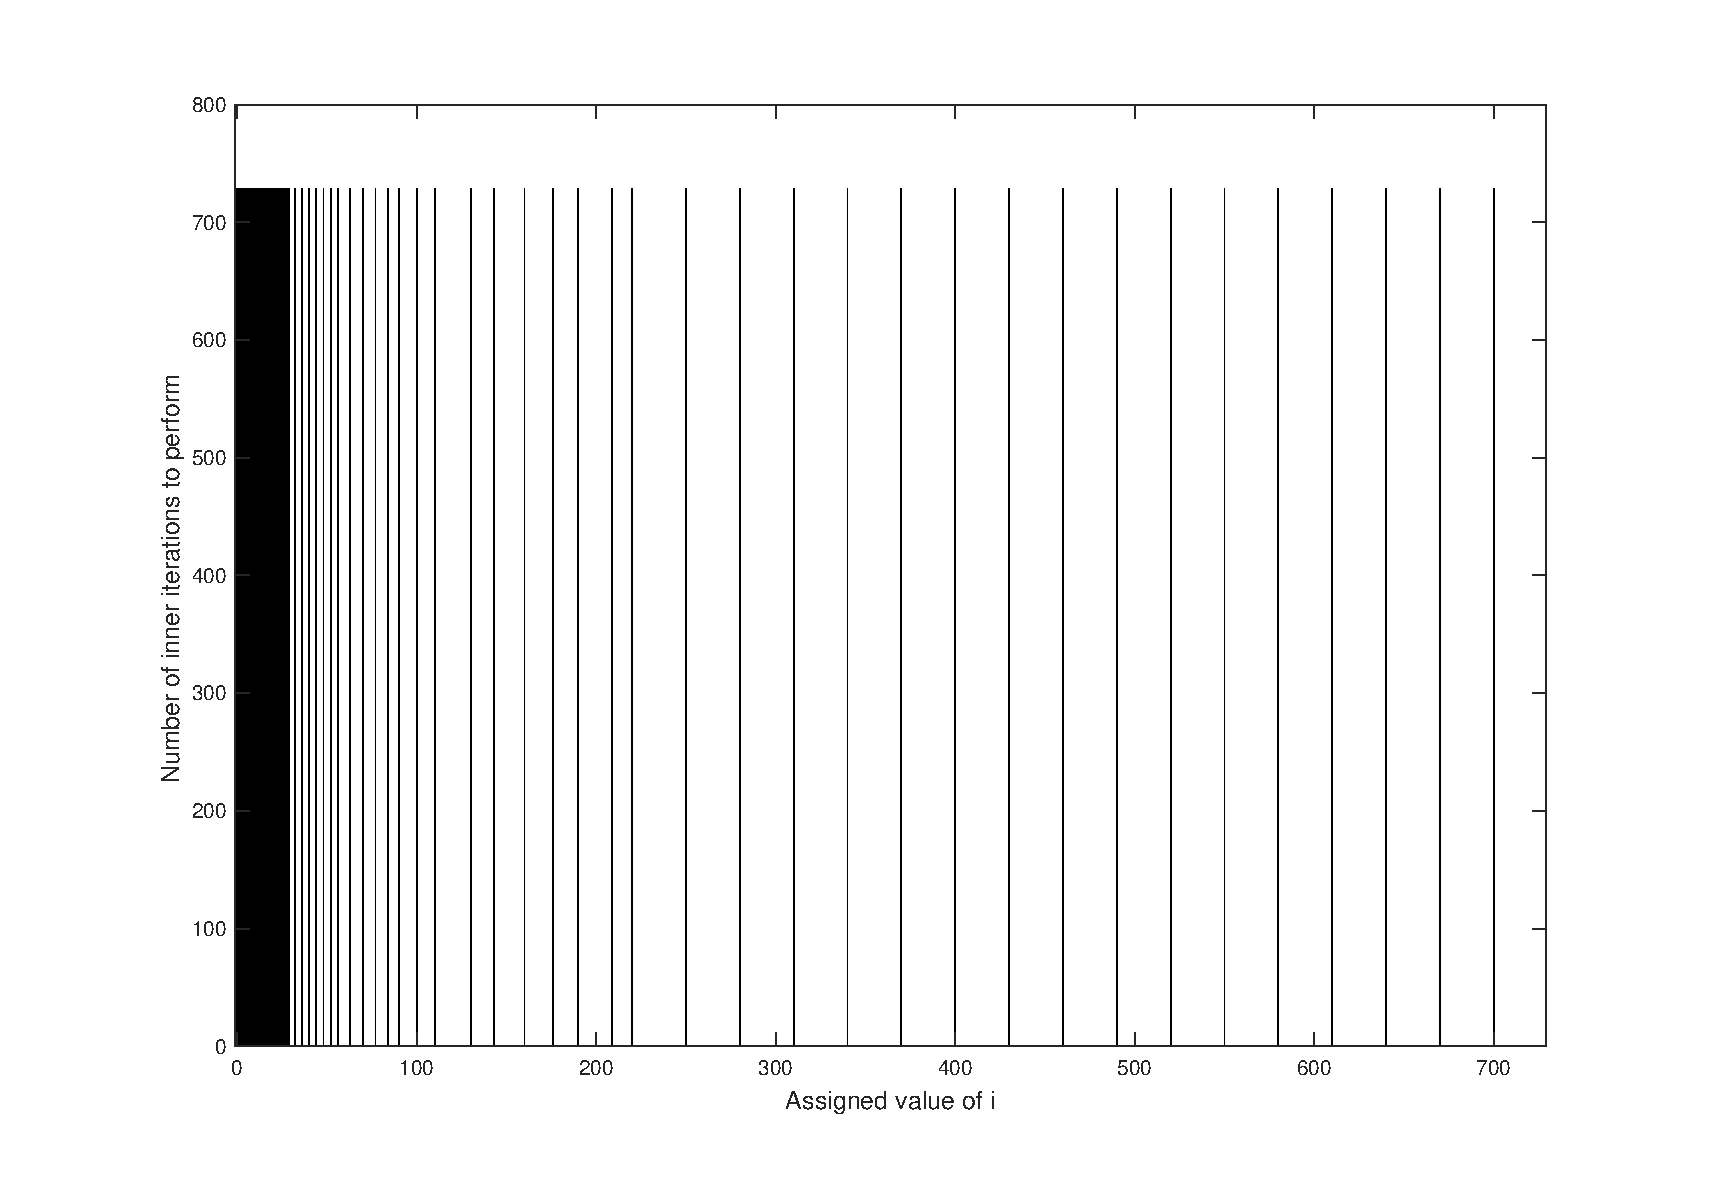
\includegraphics[width=\linewidth]{part1_plots/loop2_balancing.eps}
        \caption{The number of inner-loop iterations in Loop 2 a thread must perform based on the value of \tp{i} it is assigned; note that threads may be required to perform either $1$ or $729$ inner iterations. This is a severe work imbalance that would need to be addressed effectively to maximise performance.}
        \label{fig:loop2work}
    \end{subfigure}
\end{figure}

Loop 2 (Figure \ref{listing:loop2}), however, is a poorly-balanced loop. The \texttt{i}-th element of \texttt{jmax} is initialised to either $1$ or $N$, depending on the value of \texttt{i}.
As a result, a thread which is assigned the work of a value of \texttt{i} equal to $N$ will perform far more work than the threads with only $1$ inner iteration to compute (Figure \ref{fig:loop2work}).
Loop scheduling algorithms that are suitable for loops with widely fluctuating work levels, such as DYNAMIC or GUIDED, would be expected to work well here.

Maximising loop performance can be seen as minimising the total idle time for threads: the more time each thread spends on computing the solution, the better our performance will be.

\section*{OpenMP-standard Scheduling Algorithms}

The scheduling algorithms included in the OpenMP standard were considered first.
Loop 1 and Loop 2 represent `embarassingly parallel' problems, and as such, parallelising the routines was relatively trivial: both loops were enclosed in a \tp{!\$OMP PARALLEL DO} construct, and set such that their arrays were shared (as well as \tp{rN2} in the case of Loop 2), with all other variables set private.
The scheduling algorithm was then set to be allocated at runtime -- \tp{SCHEDULE(RUNTIME)} -- and the associated \tp{OMP\_RUNTIME} environment variable was exported to the compute node at job submission, which was controlled by a lightweight governing bash script that would parametrically generate the PBS submission file for every possible combination of scheduling algorithm and chunk size. The program was designed to take in the number of threads to use as a command line argument to the program execution. The results of an \tp{OMP\_GET\_SCHEDULE} call as part of the main Fortran program were printed to the screen to ensure the correct scheduling algorithms; the call returns an integer of type \tp{omp\_schedule\_kind} that can be cross-checked against the scheduling kinds contained in the \tp{omp\_lib\_kinds} module as part of \tp{libgomp}.

% \begin{figure}
%     \centering
%     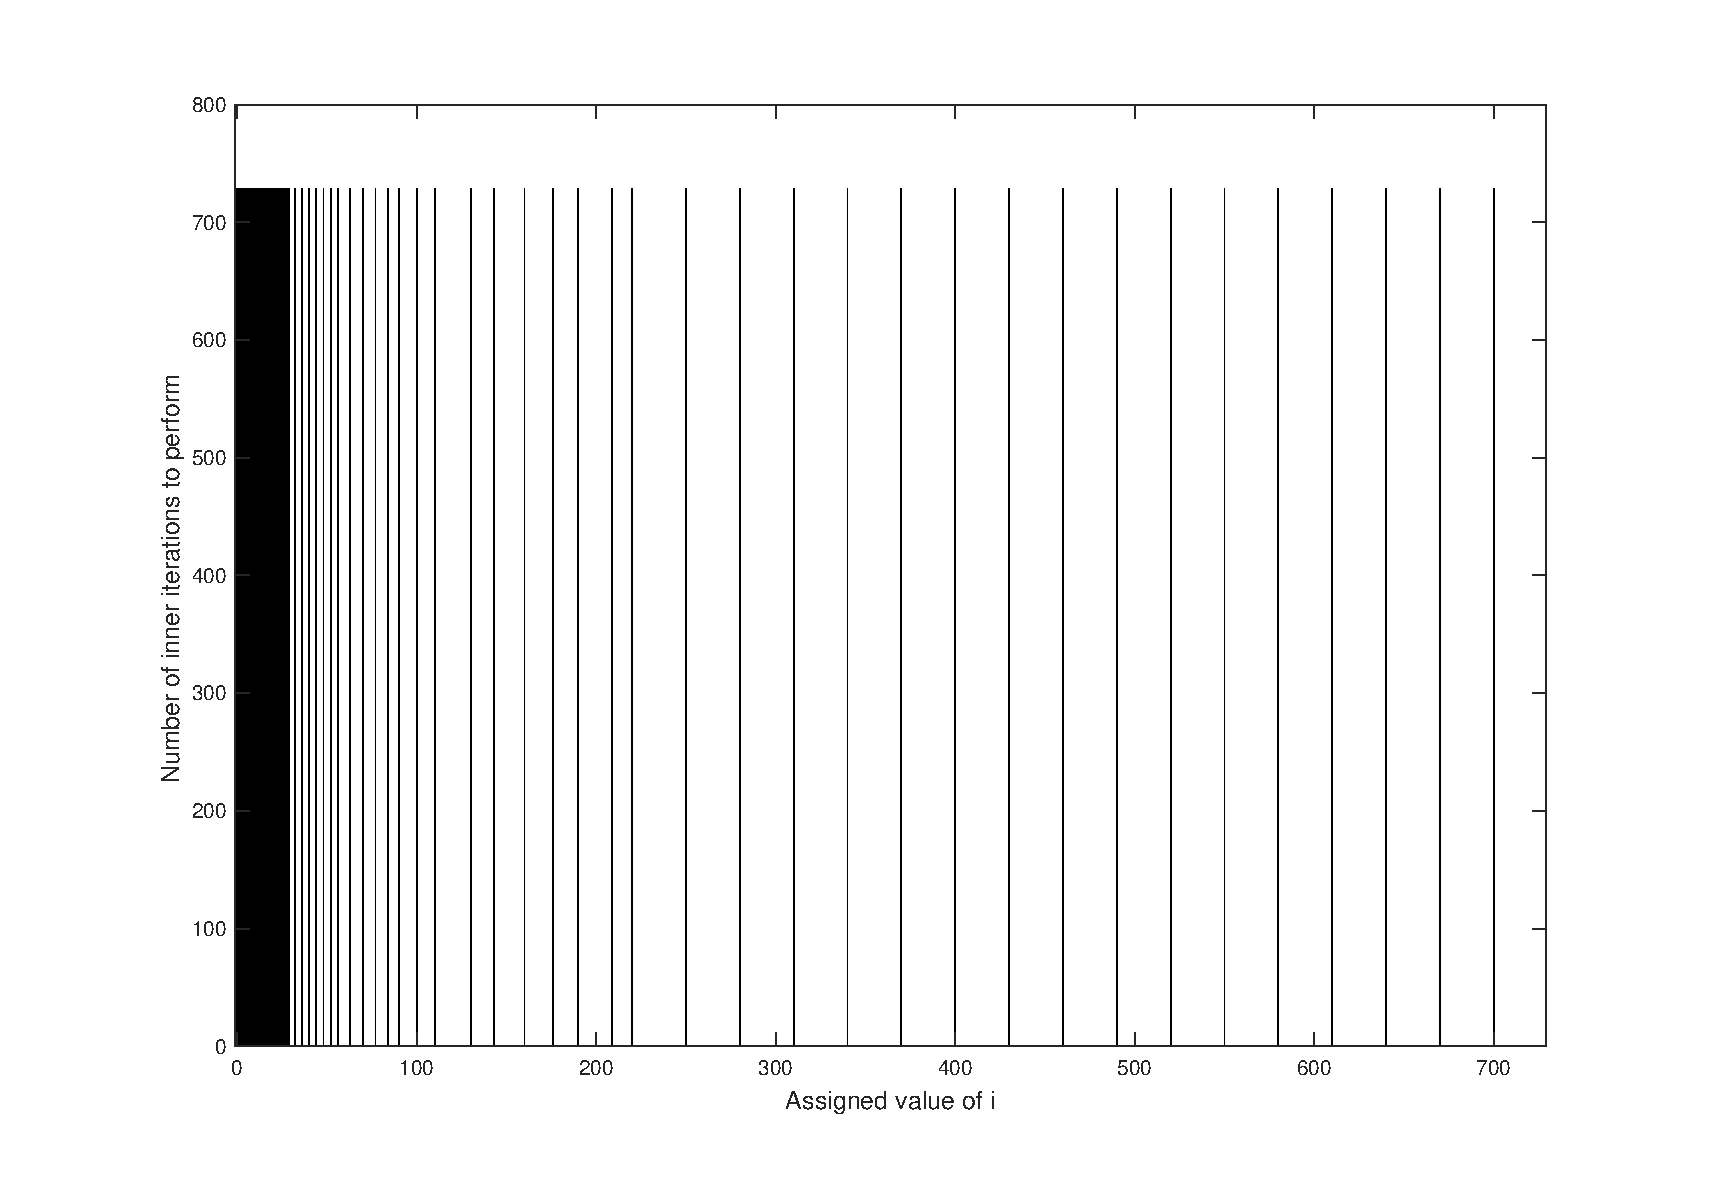
\includegraphics[height=.35\textheight]{part1_plots/loop2_balancing.eps}

% \end{figure}

\begin{figure}
    \begin{lstlisting}
        do i = 1,N

            do j = 1, jmax(i) 
        
                do k = 1,j 
                    
                    c(i) = c(i) + k * log(b(j,i)) * rN2
                
                end do
            
            end do
     
        end do
    \end{lstlisting}
    \caption{Loop 2; note that this loop is poorly-balanced as a result of the inner loop being iterated to either $1$ or $N$, depending on the value of \texttt{i}.}
    \label{listing:loop2}
\end{figure}

Submitting all of the jobs as a batch also meant that the timing results were more accurate, as jobs were almost-guaranteed to be computed on the same node.
Each job was also repeated five times, and an average taken, to further remove the effects of variable computational performance on each run.

The results for Loop 1 are given in Figure \ref{fig:loop1results}. Clearly, the \tp{AUTO} scheduling performs worse than the serial case (note that, while the AUTO execution time has been extended across all chunk sizes, the chunk size was not specified and this has been done for clarity only.)
It is not immediately clear why this scheduling option performs this poorly, as there is no transparency in the scheduling implemented, but it is clear that this option should be avoided here.
Interestingly, the performance of the \tp{STATIC, \textit{n}} scheduling routine decreases with increases in chunk size.
This is to be expected, and highlights the poor work-balancing of the loop; when threads are assigned contiguous chunks of $n$ iterations to perform, then the first threads will always perform more work than the final threads, due to the distribution of iterations (Figure \ref{fig:loop1work}).
For low chunk sizes, the high-work loops is relatively well-distributed amongst all threads, and thus there is relatively little idling and generally decreased performance time.
However, when high chunk sizes are used, the first thread takes the majority of the work, and thus acts as a bottleneck for the program execution. 
The higher the chunk size, the longer the final threads are idling waiting for the first thread(s) to finish.

The performance of most of the routines with chunk size $1$ scheduling routine is also worse than the serial version. This highlights the scheduling overheads of OpenMP; the additional time to schedule and distribute work can introduce significant performance issues.

As expected, \tp{DYNAMIC} and \tp{GUIDED} perform well for this loop.
Since \tp{DYNAMIC} assigns chunks of loop iterations to threads on a first-come, first-served basis, at small chunk sizes threads which are initially assigned less work will be assigned more work whilst other threads are still computing. 
\tp{GUIDED} functions similarly, but the loop iterations start off large and get expontentially smaller: thus, for loops with initially high amounts of work, such as this, we would expect good performance.

\begin{figure}
    \centering
    \includegraphics[height=.35\textheight]{part1_plots/all_part1.eps}
    \caption{Loop 1 execution performance for different scheduling algorithms: \tp{DYNAMIC\textit{2}} provides the best performance here overall, but \tp{GUIDED} performs better across a wider range of chunk sizes.}
    \label{fig:loop1results}
\end{figure}

Indeed, \tp{DYNAMIC,2} produces the best performance for this problem, with an execution time of $0.03449$s; with low chunk sizes, the difference between \tp{GUIDED}'s exponentially smaller, and \tp{DYNAMIC} constant, iteration allocations, may be negligible.
However, with reference to Figure \ref{fig:loop1results}, \tp{DYNAMIC} has variable performance for varying chunk sizes, with \tp{GUIDED} having generally superior performance across all chunk sizes.
\tp{GUIDED}'s scheduling matches the load-balancing well for this problem, and has a performance decrease from the optimum of only $.23\%$.
Therefore, while \tp{DYNAMIC,2} is the fastest scheduling choice here, \tp{GUIDED} may prove to be more versatile.

The results are relatively similar for Loop 2, and are provided in Figure \ref{fig:loop2results}. 
Again, the \tp{AUTO} scheduling performs poorly, and routines with chunk size $1$ perform worse than the serial case.

Because of the unusual loading in this loop, the first 30 iterations are required to do the maximum amount of work.
Therefore, scheduling algorithms that spread this initial work out across threads would reduce idling times for the unloading threads and thus increase performance.
This explains the behaviour of many of the scheduling algorithms above: when the chunk size begins to increase -- in the case of \tp{DYNAMIC} and \tp{GUIDED}, the minimum chunk size -- then fewer threads get assigned the initial amounts of work.
While the \tp{DYNAMIC} and \tp{GUIDED} algorithms will compensate somewhat, by allowing threads that would otherwise be idle to be re-assigned work, the additional loads spaced 30 iterations apart will prevent threads from idling often and being re-assigned work.

\begin{figure}
    \centering
    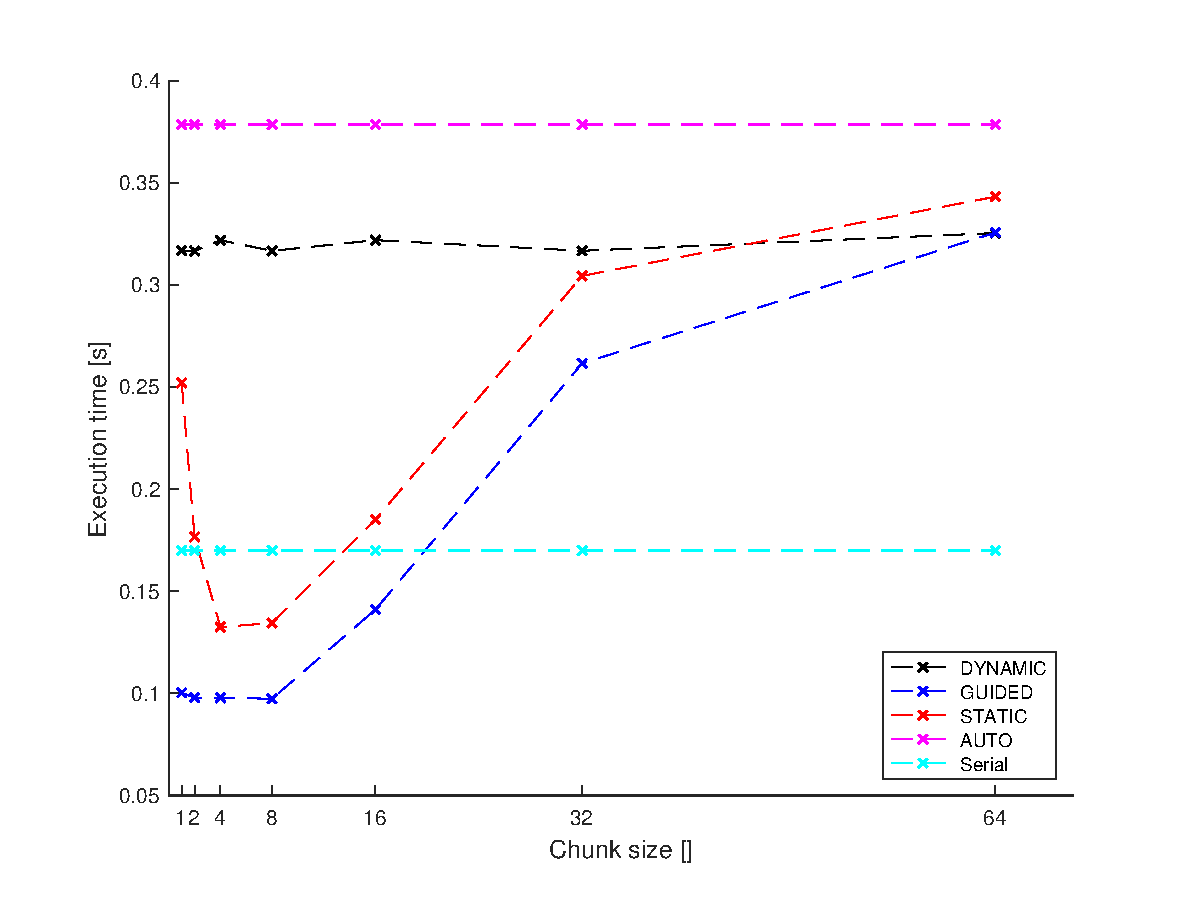
\includegraphics[height=.35\textheight]{part1_plots/all_part2.eps}
    \caption{Loop 2 execution performance for different scheduling algorithm. \tp{GUIDED,8} provides the best performance for Loop 2, but performance generally reduces with increasing chunk size.
    This is a quirk of the unusual loading for Loop 2.}
    \label{fig:loop2results}
\end{figure}

Interestingly, \tp{DYNAMIC} has constant performance for all chunk sizes; this may suggest that, since the chunk size passed to the scheduler specifies only the minimum chunk size used, the algorithm is using only large chunk sizes.

\tp{GUIDED}, and specifically \tp{GUIDED,8}, has the best execution time for this problem. This is again expected, with \tp{GUIDED} allowing threads with low amounts of work to accept work from other threads, and also forcing the latter portions of the loop iterations to be assigned in exponentially smaller chunks, spready the workload better.

As expected, however, the performance of both \tp{GUIDED} and \tp{STATIC} reduce with increases in chunk size.

Fastest method for loop 1: DYNAMIC,2

Fastest method for loop 2: GUIDED,8


\section*{Affinity Scheduling}

In view of the performance of the OpenMP-standard loops, attention now turns to an implementation of static partitioned affinity scheduling, an algorithm developed by \citet{273046}.
The algorithm is designed for parallel loops nested inside serial loops, and aims to ensure that cache misses and processor idling times are minimised.

The algorithm functions by allocating an equal proportion of the total work to each thread. 
When a thread finishes each of its initial allocation, it will `steal' work from the thread with the most remaining of its initial allocation.

Much of the algorithm's speed comes from the determinstic loop allocation at the initial execution of the loop, which ensures that the $i$th processor holds the $i$th chunk of iterations.
By doing so, the data required for repeated executions of the loop will already be stored in cache, removing the need for relatively expensive memory movements.
Also, the algorithm assumes, at first, that the loop is perfectly balanced, and therefore takes initially large chunks of work.
Thus, there is only a scheduling overhead at the beginning of the loop.

When each thread does finish its local thread, work is reassigned to smooth the load imbalance and prevent threads from idling.
By only reassigning at the point of imbalance, unlike \tp{DYNAMIC} or \tp{GUIDED} which begin to perform large re-scheduling in the latter portions of the loop, the scheduling and memory re-allocation overhead is only incurred when required, and memory is moved at most twice when work is reallocated.

\subsection*{Implementation}

A description of the behaviour of the algorithm, and its' implementation, follows:

Each thread is initially assigned $P/N$ iterations, where $P$ is the total number of iterations and $N$ the number of threads. 
Should $N$ not divide evenly into $P$, then the remainder $r$ is scattered across the first $r$ threads.
The number of iterations each thread is to perform is stored in an array indexed by the thread identifier retrieved from \tp{OMP\_GET\_THREAD\_NUM}.
Since this array must be shared in the parallel region, the synchronisation of, and access to, the array must be closely controlled.
\tp{CRITICAL} sections or \tp{LOCK}s must be implemented to prevent race conditions and unintended overwrites.
A discussion on this is given in Section \ref{s:locks}.

Other shared variables, such as the number of threads, and the value of $P/N$, are also shared.
By default, all other variables are scoped as \tp{PRIVATE} in all parallel regions.

At this point, each thread is begins work on $1/P$ iterations of its initial assignment, and updates the (shared) number of iterations array to announce to the other threads that it has taken those iterations to be executed.
This contiguous assignment ensures that repeated iterations will access data already stored in local caches.

This assignment is again enclosed in either a \tp{CRITICAL} region, or \tp{LOCK}s are used to prevent race conditions on each element of the array.
From here forwards, the number of iterations array tracks the number of iterations remaining for each thread.

The upper and lower bounds of iteration counter are then determined parametrically from the thread identification number and the number of iterations remaining; the algorithm starts at the `bottom' of each thread's chunk and moves upward.

In order to aid the execution of this type of scheduling algorithm, the \tp{loop1} and \tp{loop2} subroutines now take in two \tp{integer}-type arguments, that set the upper and lower bounds for the outer loop.
Owing to the variable scoping in the internal procedures in Fortran, the shared arrays \tp{a}, \tp{b} and \tp{c} may be accessed without specification of their OpenMP scope.

This process is repeated for all threads until one or more completes its initial assignment of threads.
At this point, it is likely, especially in imbalanced loops, that other threads will still be working.
So as to minimise idling times, each `finished' processor -- that is, one that has completed its initial assignment -- will use the array of remaining iterations to determine which other thread is currently the most loaded.
The finished thread will then `steal' work from the most loaded thread, appropriately emunlating the thread identifiers of the most loaded thread to properly update the shared arrays to announce to other threads that it has taken some of the loaded thread's iterations to be executed.
So that no two finished threads are assigned the same work, \tp{CRITICAL}s or \tp{LOCK}s are used again.

When all threads have finished their local assignment, the loop has completed.

\subsection*{Results: Affinity Scheduling}

\begin{figure}
    \centering
    \includegraphics[width=.8\textwidth]{part2_plots/affinity_loop1}
    \caption{Execution times for Loop 1, scheduled using the static partitioned affinity scheduling algorithm. We obtain better performance as we increase the number of threads, until the array chunks no longer fit in the processor cache.}
    \label{fig:affinityloop1}
\end{figure}

\begin{figure}
    \centering
    \includegraphics[width=.8\textwidth]{part2_plots/affinity_loop2}
    \caption{Execution tiems for Loop 2, scheduled using the static partitioned affinity scheduling algorithm. Again, we obtain better performance as we increase the number of threads, although the performance does not scale one-to-one with the number of threads.}
    \label{fig:affinityloop2}
\end{figure}


\subsection*{\tp{CRITICAL} vs. \tp{LOCK}s}\label{s:locks}

We may define two distinct types of self-scheduling -- where each thread is responsible for seeking more work -- algorithms: fixed, and variable.
Where, in fixed systems, each processor will thread will perform a fixed amount of work whenever it sets to be idle, variable algorithms choose initially large amounts of work , but take increasingly small amounts of work as iterations progress.
Self-scheduling algorithms, such as the \tp{STATIC} directive, can be inappropriate for low chunk-size loops, where the scheduling overhead can dominate execution times \citep{1701915}.
Alternatively, where each processor takes $\frac{1}{N}$ of the loop iterations, where $N$ is the number of threads, the scheduling is unable to adjust to imbalances in work present in each portion of the loop.

Variable algorithms that take initially large amounts of work reduce the overhead required for scheduling \citep{Eager1992AdaptiveGS, Polychronopoulos:1987:GSP:40938.40941}.
However, by taking small amounts of work towards the end of the loop, these algorithms may offer performance for imbalanced loops, since these small chunk sizes may smoothen the differences in work from the initial assignments.

Another significant impact on loop performance is associated with memory caching; by ensuring that the same data is used repeatedly, the overheads of moving data from main memory to processor memory can be avoided.

Our qualitative performance metrics are thus scheduling methods that allow data to be worked on in relatively large, contiguous chunks, and scheduling methods that reduce the total idling times for threads.

ahf`sdbjkzsbjgbjzsbfg

\bibliographystyle{plainnat}

\newpage
\bibliography{bib.bib}

\end{document}
